% Tikz File 'mytikz.tex'
\documentclass{standalone}
\usepackage{tikz}
%\usetikzlibrary{...}
\begin{document}
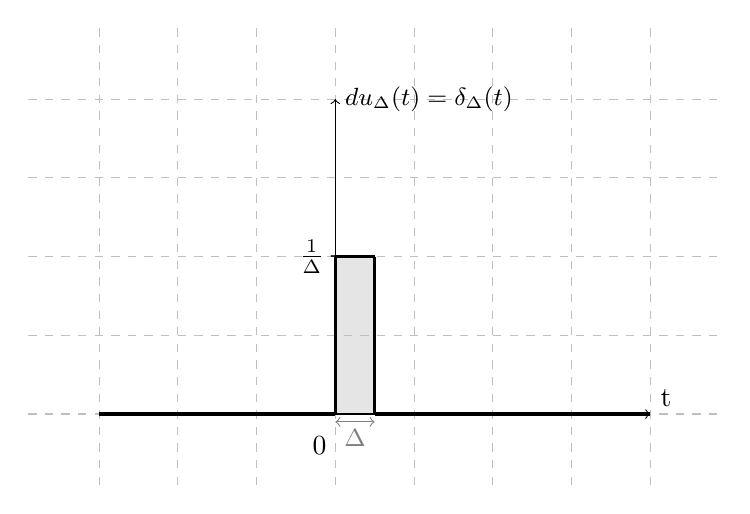
\begin{tikzpicture}
    % Fill the area under the curve
    \fill[gray!20] (0,0) -- (0,2) -- (0.5,2) -- (0.5,0) -- cycle;

    % Add grid
    \draw[gray!50, dashed, step=1] (-3.9,-0.9) grid (4.9,4.9);

    % Add axes
    \draw[->] (-3,0) -- (4,0);
    \draw[->] (0,0) -- (0,4) node[right] {\small $du_{\Delta}(t) = \delta_{\Delta}(t)$};
    \node at (0,2) {-};
    \node at (-0.3,2) {$\frac{1}{\Delta}$};

    % labels for x-axis
    \node at (4.2,0.2) {t};
    \node at (-0.2,-0.4) {0};

    % create the unit step function in continuous time
    \draw[-, very thick] (-3,0) -- (0,0);
    \draw[-, very thick] (0,0) -- (0,2);
    \draw[-, very thick] (0,2) -- (0.5,2);
    \draw[-, very thick] (0.5,2) -- (0.5,0);
    \draw[-, very thick] (0.5,0) -- (4,0);

    \draw[<->, gray] (0,-0.1) -- (0.5,-0.1) node[midway, yshift=-0.2cm] {\small $\Delta$};

\end{tikzpicture}
\end{document}


